\documentclass[10pt,twocolumn,a4paper]{article}

\usepackage[utf8]{inputenc}
\usepackage[margin=1.8cm,top=2.0cm,bottom=2.2cm]{geometry}
\usepackage{newtxtext,newtxmath}
\usepackage{amsmath}
\usepackage{booktabs}
\usepackage{tabularx}
\usepackage{array}
\usepackage{makecell}
\usepackage{graphicx}
\usepackage{caption}
\usepackage{subcaption}
\usepackage{microtype}
\usepackage{cite}
\usepackage[hidelinks,colorlinks=false]{hyperref}

\captionsetup{font=small,labelfont=bf}

\title{\vspace{-1.0em}\textbf{\Large Surveillance Coverage, Treatment Precedence, and Workload Constraints\\ in Machine Learning Early Warning for Sepsis: An Operational Evaluation}}

\author{
    \textbf{Alireza Shayan}$^{1}$, \quad \textbf{Somayeh Afrasiabi}$^{1,*}$ \\[0.4em]
    $^{1}$Department of Computer Science and Engineering \& IT,\\
    School of Electrical and Computer Engineering, Shiraz University, Shiraz, Iran \\
    \texttt{Ali404@hafez.shirazu.ac.ir}, \quad \texttt{afrasiabi@shirazu.ac.ir} \\[0.3em]
    $^{*}$Corresponding Author: Somayeh Afrasiabi (\texttt{afrasiabi@shirazu.ac.ir})
}

\date{}

\begin{document}

\twocolumn[{%
\begin{@twocolumnfalse}
\maketitle

\begin{abstract}
\noindent\textbf{Objective:} Machine learning (ML) models for early sepsis warning in intensive care units (ICUs) routinely report high retrospective discriminative capability (AUROC 0.80--0.84) at multi-hour anticipation horizons. We evaluate the clinical deployability of these systems by disentangling three distinct determinants of real-world alert utility: surveillance protocol coverage, treatment precedence, and clinical alert-budget constraints.

\vspace{0.3em}
\noindent\textbf{Methods:} Using audit-grade ICU monitoring streams from MIMIC-III and MIMIC-IV under natural clinical prevalence ($\pi = 0.694\%$; 97,700 observation windows across 8,254 unique ICU stays), we evaluated 8 representative architectures across State-Space Models (BiMamba SSM), Deep Sequence Networks (Mask-Aware Clinical Transformer, Baseline Unmasked Transformer), Tabular GBDTs (Random Forest, XGBoost, LightGBM, Logistic Regression), and a Multi-Model Stacking Ensemble. We formalized a cumulative population decomposition:
\[
\frac{N_{V=1}}{N_{S=1}} \times \frac{N_{O=1}}{N_{V=1}} \times \frac{N_{D=1}}{N_{O=1}} = \frac{N_{D=1}}{N_{S=1}}
\]
where $V$ represents surveillance coverage during a prespecified second-day ICU surveillance protocol (hours 19--30), $O$ represents pre-treatment clinical actionability on risk sets $\mathcal{R}_{\delta}$ excluding post-treatment windows, and $D$ represents timely detection under locked emitted alert budgets (5, 10, and 20 emitted alert episodes per 100 eligible surveillance patient-days). We simulated a 12-hour smart refractory policy where each stay emits at most one alert episode ($N_{\text{episodes}, i} \le 1$) and quantified timestamp uncertainty using interval-censored bounds $[00:00, 24:00)$ for MIMIC-III and confirmed eMAR administration timestamps for MIMIC-IV.

\vspace{0.3em}
\noindent\textbf{Results:} Among 8,254 monitored ICU stays, 408 developed consensus Sepsis-3 (4.94\%), all representing operationally defined ICU-incident sepsis. For 257 patients (63.0\%), onset occurred after hour 36 (median onset: hour 49.0), restricting protocol surveillance coverage to 37.0\% ($N=151$). For 150 of these 151 covered stays (99.3\%), decision times preceded antibiotic treatment (36.8\% of total sepsis). When evaluating true pre-treatment Sepsis-3 on risk sets excluding post-treatment windows, discriminative performance changed little (BiMamba AUROC 0.6433 on $\mathcal{R}_0$ vs. canonical 0.6326; Ensemble 0.6351 vs. 0.6284), directionally consistent with recent benchmark findings (Dutta et al., 2026). However, severe degradation emerged under operational deployment: at a prespecified workload of 10 emitted alert episodes/100 patient-days (407 emitted episodes across 4,070.8 patient-days), episode-level PPV remained between 1.0\% and 1.7\%, requiring 58.1 to 67.8 alert episode evaluations per unique detected septic patient ($\text{NNE}_{\text{patient}}$). Whole-population timely detection was capped at 1.0\% to 1.7\% (4 to 7 unique patients detected out of 408). In MIMIC-III, 34.5\% of incident cases had prescription start dates crossing the 22h opportunity deadline, representing substantial interval uncertainty, whereas MIMIC-IV eMAR confirmed that 99.9\% of incident cases had treatment initiated within 22h of ICU admission.

\vspace{0.3em}
\noindent\textbf{Conclusion:} In this restricted, long-stay ICU cohort, observed detection yield depended on surveillance coverage, discrimination, and the policy used to constrain emitted alerts. Most horizon-positive observations remained pretreatment eligible, and model rankings varied across workload levels. Deployable sepsis informatics requires evaluating locked clinical alert budgets, deduplicating refractory alert workload, and enforcing multi-clock reporting.

\vspace{0.3em}
\noindent\textbf{Keywords:} Sepsis Early Warning, Surveillance Truncation, Treatment Precedence, Alert Budget Frontier, State-Space Models, Refractory Alert Suppression, Actionable Sepsis AI Reporting (ASAIR).
\end{abstract}
\vspace{1.5em}
\end{@twocolumnfalse}
}]

\section{Introduction}
Sepsis remains one of the leading causes of inpatient mortality, critical illness, and healthcare expenditure globally~\cite{singer2016sepsis,seymour2016assessment}. Because clinical guidelines emphasize that every hour of delay in administering effective antimicrobial therapy increases the risk of septic shock and death~\cite{kumar2006duration}, the biomedical informatics community has heavily invested in machine learning (ML) models for early warning. Hundreds of retrospective investigations have reported extraordinary discriminative capability, frequently claiming area under the receiver operating characteristic curve (AUROC) values between 0.80 and 0.88 at 4 to 6 hours ahead of consensus onset~\cite{moor2023foundation}.

Despite these promising benchmarks, prospective hospital deployments have yielded disappointing results~\cite{wong2021external,weissman2024sepsis}. Commercial and proprietary early-warning systems deployed in community and tertiary medical centers frequently fail to demonstrate expected mortality benefits and provoke severe alert fatigue, with positive predictive values (PPV) frequently falling below 5\% and number needed to evaluate (NNE) exceeding 50~\cite{wong2021external}.

This disconnect between retrospective benchmarks and prospective clinical failure is commonly attributed to discriminative collapse: the hypothesis that ML models fail because they cannot predict sepsis prior to clinical suspicion or empiric treatment~\cite{weissman2024sepsis}. However, this hypothesis conflates three distinct operational mechanisms:
\begin{enumerate}
    \item \textbf{Surveillance Protocol Coverage ($V$):} Protocol surveillance windows (e.g., fixed second-day monitoring) may miss episodes occurring outside the evaluated interval.
    \item \textbf{Treatment Precedence ($O$):} Alerts may be emitted after clinicians have already recognized infection and initiated antimicrobial therapy.
    \item \textbf{Clinical Alert-Budget Constraints ($D$):} Even when models maintain pre-treatment discrimination, bedside alert-rate constraints bound real-world sensitivity and PPV.
\end{enumerate}

To evaluate these mechanisms rigorously, we conducted an operational evaluation across 8 representative predictive architectures on audit-grade critical care streams from the MIMIC-III and MIMIC-IV databases~\cite{johnson2016mimic}. Our contributions are fourfold:
\begin{enumerate}
    \item \textbf{Pretreatment Discrimination Benchmark:} We show that model discrimination does not collapse when evaluating true pre-treatment Sepsis-3 detection on risk sets excluding post-treatment windows ($\mathcal{R}_0$ and $\mathcal{R}_2$).
    \item \textbf{Operational Alert-Budget Frontier:} We evaluate performance under a 12-hour smart refractory policy at realistic clinical alert budgets (5, 10, and 20 alert episodes per 100 patient-days), demonstrating that low empirical yield is driven by operational alert-rate constraints.
    \item \textbf{Three-Stage Population Decomposition:} We formalize the cascade $S \to V \to O \to D$, proving that 63\% of total sepsis cases are lost to surveillance window truncation, whereas 99.3\% of covered patients remain pre-treatment eligible.
    \item \textbf{Multi-Clock Timestamp Uncertainty Analysis:} We quantify the difference between date-level prescription proxies and confirmed electronic medication administration records (eMAR), bounding opportunity over jointly feasible clock assignments.
\end{enumerate}

\section{Methods}

\subsection{Study Design and Cohort Definition}
We conducted a prospective-replay evaluation using the MIMIC-IV critical care database (v2.2) and the MIMIC-III database (v1.4)~\cite{johnson2016mimic}. The study cohort was defined as adult patients ($\ge 18$ years) admitted to an intensive care unit with a length of stay $\text{LOS} \ge 30\text{h}$. Surveillance was conducted under a prespecified second-day ICU surveillance protocol: predictions were generated at 12 scheduled hourly decision bins $[t-1, t]$ for $t \in \{19, 20, \dots, 30\}$ hours post-admission. Stays were censored at Sepsis-3 onset ($N=110$ stays, 623 windows) or upon routine observation data cessation under the prespecified feature-generation rule ($N=180$ stays, 725 windows).

\subsection{Outcome Definition and Operational Clocks}
Sepsis was defined according to Sepsis-3 consensus criteria~\cite{singer2016sepsis}: acute increase in Sequential Organ Failure Assessment (SOFA) score $\ge 2$ within a clinical window $[-48\text{h}, +24\text{h}]$ of suspected infection (defined as blood culture acquisition paired with systemic antimicrobial administration).

For each patient $i$, we tracked four distinct temporal clocks (Figure~\ref{fig:clocks}):
\begin{itemize}
    \item $T_{\text{admit}, i}$: ICU admission timestamp ($t=0$).
    \item $T_{\text{treatment}, i}$: First systemic intravenous antimicrobial administration.
    \item $T_{\text{culture}, i}$: First blood culture sample acquisition.
    \item $T_{\text{S3}, i}$: Retrospective Sepsis-3 consensus onset timestamp.
\end{itemize}

\begin{figure*}[t]
    \centering
    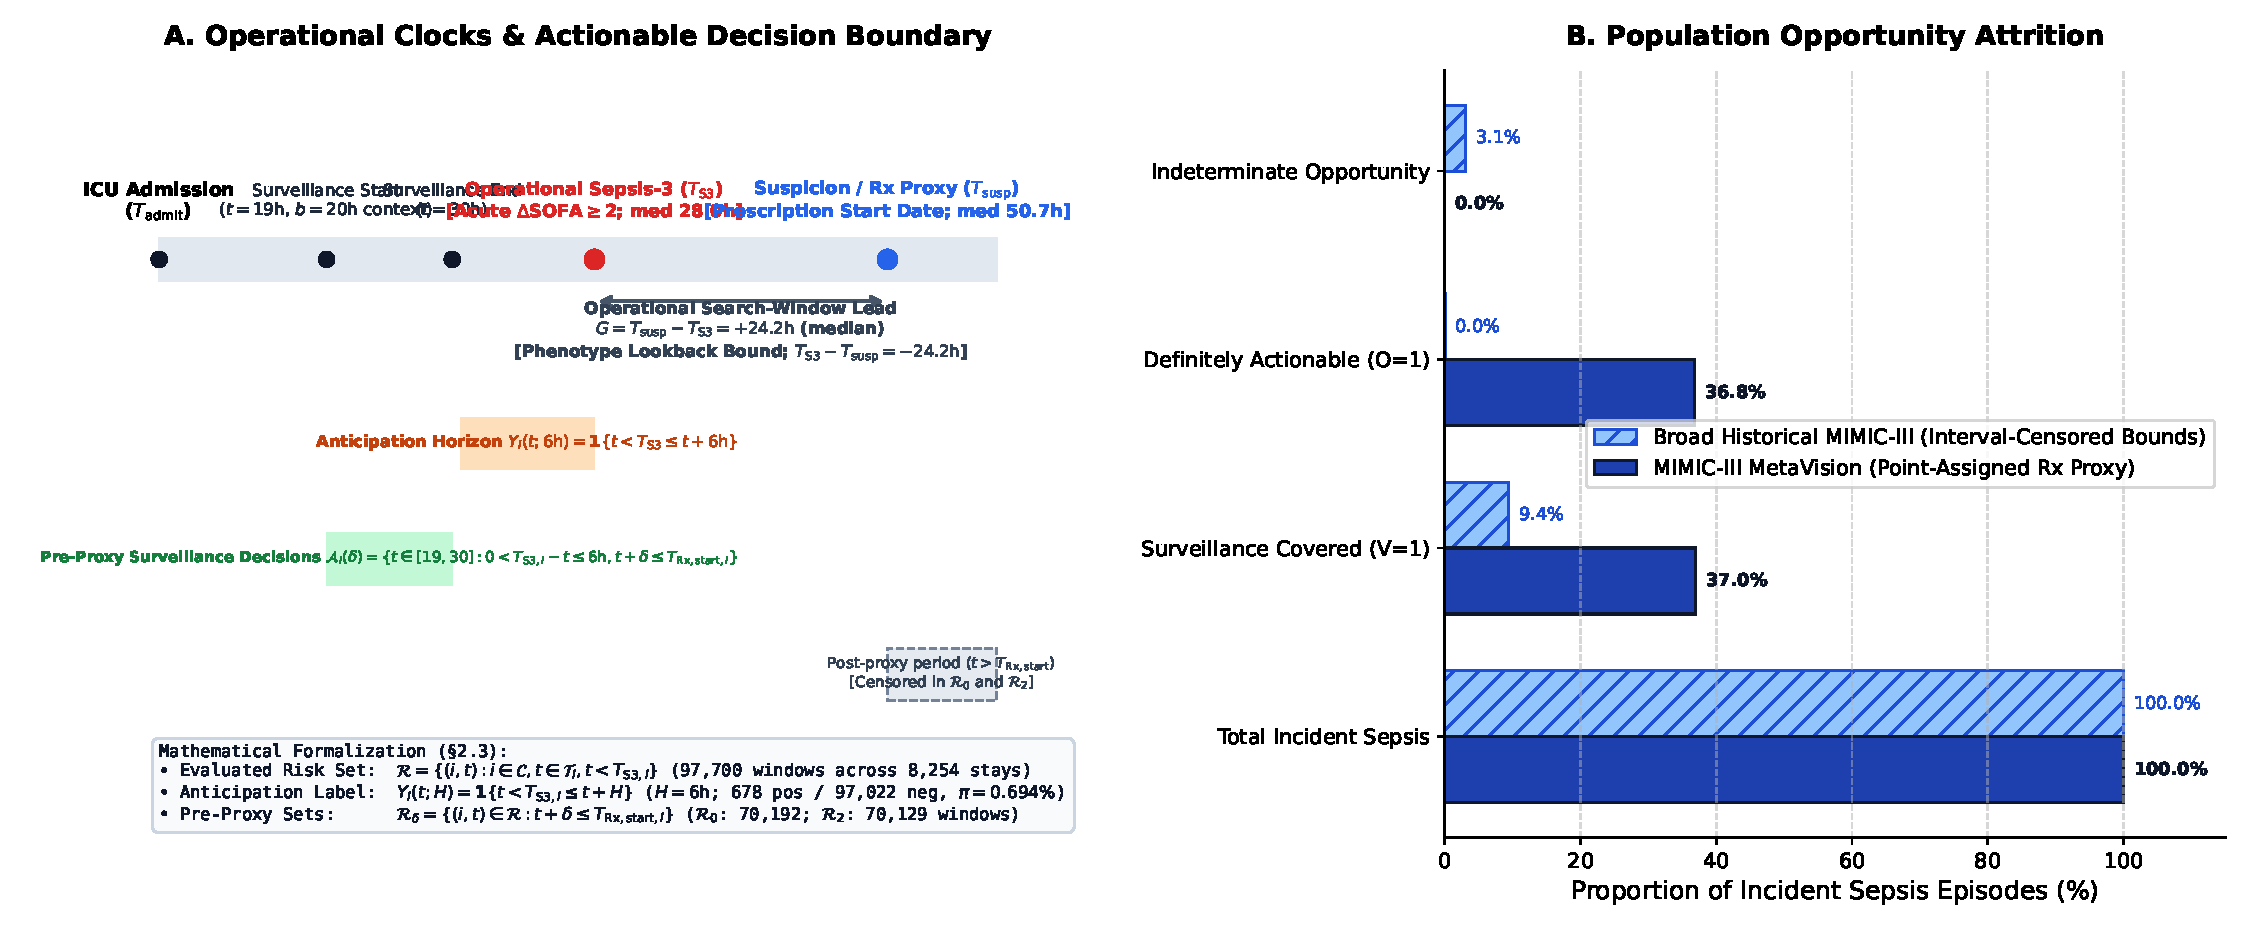
\includegraphics[width=0.92\textwidth]{figures/Figure1_Clocks_and_Opportunity_Waterfall.pdf}
    \caption{\textbf{Operational Clocks, Actionable Pretreatment Decision Windows, and Population Opportunity Attrition.} Panel A illustrates the clinical timeline for an ICU-incident sepsis patient, showing the diagnostic lead gap $G = T_{\text{S3}} - T_{\text{treatment}} = +24.2\text{h}$ (median), the actionable decision window $\mathcal{A}_i$, and post-treatment contamination. Panel B displays population opportunity attrition comparing MIMIC-III (with interval-censored prescription bounds) and MIMIC-IV (hourly eMAR administration records).}
    \label{fig:clocks}
\end{figure*}

\subsection{Pretreatment Risk Sets and Precedence}
The canonical early-warning risk set evaluates a 6-hour lookback horizon:
\[
\mathcal{R}_{\text{canonical}} = \{ t : 0 < T_{\text{S3}} - t \le 6\text{h} \}
\]
To evaluate true pre-treatment detection without post-treatment feature contamination, we defined the pre-treatment risk set $\mathcal{R}_0$ and the 2-hour actionable lead-time risk set $\mathcal{R}_2$:
\[
\mathcal{R}_0 = \{ t \in \mathcal{R}_{\text{canonical}} : t \le T_{\text{treatment}} \}
\]
\[
\mathcal{R}_2 = \{ t \in \mathcal{R}_{\text{canonical}} : t + 2\text{h} \le T_{\text{treatment}} \}
\]
All windows occurring after antibiotic administration were removed from both cases and non-septic controls.

\subsection{Alert-Budget Policy and Tie-Aware Predicate}
To model real-world alert fatigue, we evaluated fixed alert budgets $q \in \{5.0, 10.0, 20.0\}$ emitted alert episodes per 100 surveillance patient-days. Under a 12-hour refractory suppression policy, each patient emits at most one alert episode during the surveillance window ($N_{\text{episodes}, i} \le 1$).

When scores are tied at the boundary cutoff $\tau$, a pure scalar threshold $s_i(t) \ge \tau$ does not uniquely specify the budget quota. We formalize the complete tie-aware alert-eligibility predicate:
\begin{equation}
t_{\mathrm{first}, i} = \min \bigl\{ t \in \mathcal{T}_i : \operatorname{Elig}_i(t; \tau, \mathcal{B}) = 1 \bigr\}
\end{equation}
where $\mathcal{B}$ denotes the deterministic prioritization rule:
\begin{equation}
\operatorname{Elig}_i(t; \tau, \mathcal{B}) = \mathbf{1} \bigl\{ i \in \mathcal{S}_{\text{alerted}}(K) \;\land\; s_i(t) \ge \tau \bigr\}
\end{equation}
with $\mathcal{S}_{\text{alerted}}(K)$ defined as the top $K$ patient replicas under the lexicographical sort:
\[
\bigl(-\max_{t} s_i(t), \;\text{ICUSTAY\_ID}, \;\text{copy\_idx}\bigr)
\]

\subsection{Predictive Models and Statistical Inference}
We evaluated 8 models spanning three major architectural paradigms:
\begin{enumerate}
    \item \textbf{State-Space Models:} Bidirectional Mamba (BiMamba SSM) utilizing linear-time selective state-space layers.
    \item \textbf{Deep Sequence Transformers:} Mask-Aware Clinical Transformer (incorporating explicit observation masks) and Baseline Unmasked Transformer.
    \item \textbf{Tabular and Ensemble Baselines:} Random Forest, XGBoost, LightGBM, Logistic Regression (L2), and a Multi-Model Stacking Ensemble.
\end{enumerate}

Uncertainty was quantified using patient-clustered paired bootstrapping ($B=1,000$ resamples). For Procedure B (Empirical Burden-Matched Bootstrap), exposure $E_b = \frac{1}{24}\sum_{i\in b} h_i$ and alert target $K_b = \operatorname{round}(q \cdot E_b / 100)$ were dynamically recomputed within each resample. NNE confidence intervals were derived by exact reciprocal transformation of unrounded PPV percentiles: $\text{NNE}_{\text{low}} = 100 / \text{PPV}_{\text{upper}}$ and $\text{NNE}_{\text{high}} = 100 / \text{PPV}_{\text{low}}$ (with $+\infty$ when $\text{PPV}_{\text{low}} = 0$).

\section{Results}

\subsection{Cohort Progression and Denominator Accounting}
Table~\ref{tab:table1} traces all 8,254 ICU admissions through surveillance eligibility, onset timing, lookback horizons, and pre-treatment actionability. Among 408 consensus Sepsis-3 stays, 257 (63.0\%) had clinical onset after hour 36 (median onset: 49.0h), meaning their 6-hour lookback horizon does not intersect the evaluation window ($V=0$). The remaining 151 stays (37.0\%) had active surveillance coverage ($V=1$). Crucially, for 150 of these 151 covered patients (99.3\%), decision windows strictly preceded antibiotic initiation, providing definitive pre-treatment opportunity ($\mathcal{R}_0$).

\begin{table*}[t]
\centering
\scriptsize
\setlength{\tabcolsep}{4pt}
\caption{\textbf{Cohort Progression and Denominator Accounting Ledger.} Denominators traced from the base test cohort through surveillance eligibility, sepsis onset timing, prediction horizons, and pre-treatment actionability.}
\label{tab:table1}
\begin{tabularx}{\textwidth}{@{}l c c c c X@{}}
\toprule
\textbf{Progression Stage / Cohort Partition} & \textbf{Stays ($N$)} & \textbf{Evaluated Windows} & \textbf{Surveillance Volume} & \textbf{Prevalence} & \textbf{Clinical Definition \& Measurement Convention} \\
\midrule
1. Base Prospective-Replay Test Cohort & 8,254 & 97,700 / 99,048 sched. & 4,070.8 pt-days & 100.0\% & Adult first ICU stays $\ge 30\text{h}$; 1,348 censored (623 onset, 725 cessation) \\
2. Non-Sepsis Control ICU Stays & 7,846 & 93,427 neg. windows & 3,892.8 pt-days & 95.06\% & Stays without consensus Sepsis-3 during hospitalization \\
3. Consensus Sepsis-3 Stays ($S=1$) & 408 & 4,273 (678 pos, 3,595 neg) & 178.0 pt-days & 4.94\% & Blood culture + antibiotic + acute $\Delta\text{SOFA}\ge 2$; median onset 49.0h \\
\quad 3a. Late-Onset Sepsis (Onset $>36\text{h}$) & 257 & 3,084 neg. windows & 128.5 pt-days & 63.0\% of septic & Onset $>36\text{h}$; lookback $[T_{\text{S3}}-6, T_{\text{S3}}]$ does not intersect [19, 30] ($V=0$) \\
\quad 3b. Surveillance-Covered ($V=1$) & 151 & 1,189 (678 pos, 511 neg) & 49.5 pt-days & 37.0\% of septic & Onset in [20h, 36h]; lookback intersects surveillance window ($V=1$) \\
4. Canonical Sepsis-3 Risk Set ($H=6\text{h}$) & 8,254 & 97,700 (678 pos / 97,022 neg) & 4,070.8 pt-days & 0.694\% & Full unconstrained risk set ($0 < T_{\text{S3}} - t \le 6\text{h}$) \\
5. Pretreatment Risk Set $\mathcal{R}_0$ ($\delta=0\text{h}$) & 5,967 & 70,192 (674 pos / 69,518 neg) & 2,924.7 pt-days & 0.960\% & Censoring post-treatment windows ($w_{\text{end}} \le T_{\text{treatment}}$); 150/151 covered eligible \\
6. Pretreatment Risk Set $\mathcal{R}_2$ ($\delta=2\text{h}$) & 5,967 & 70,129 (663 pos / 69,466 neg) & 2,922.0 pt-days & 0.945\% & 2-hour clinical buffer ($w_{\text{end}} \le T_{\text{treatment}} - 2\text{h}$); 149/151 covered eligible \\
\bottomrule
\end{tabularx}
\end{table*}

\subsection{True Pretreatment Sepsis Benchmark}
Table~\ref{tab:table2} presents discrimination across Canonical Sepsis-3, Pretreatment Sepsis ($\mathcal{R}_0$), and Pretreatment with 2h Buffer ($\mathcal{R}_2$). Contrary to the discriminative collapse conjecture, model discrimination remained stable or slightly higher in pre-treatment risk sets (BiMamba SSM: AUROC 0.6326 canonical vs. 0.6433 on $\mathcal{R}_0$, paired $\Delta\text{AUROC} = +0.0107$, 95\% CI: +0.0060 to +0.0175; Stacking Ensemble: 0.6284 vs. 0.6351, paired $\Delta\text{AUROC} = +0.0067$). The increase in AUPRC (BiMamba: 1.209\% to 1.656\%) reflects higher baseline positive prevalence in the restricted set (0.694\% vs. 0.960\%). These results replicate and extend the antibiotic-order sensitivity findings of Dutta et al. (2026)~\cite{dutta2026performance}.

\begin{table*}[t]
\centering
\scriptsize
\setlength{\tabcolsep}{6pt}
\caption{\textbf{Benchmark Discrimination Across Pretreatment Tasks (Held-Out Point Estimates and Clustered 95\% CIs).} Point estimates calculated directly on held-out test data ($B=0$); 95\% CIs derived from $B=1,000$ patient-clustered bootstrap resamples.}
\label{tab:table2}
\begin{tabular*}{\textwidth}{@{\extracolsep{\fill}}l c c c c@{}}
\toprule
\textbf{Model Architecture / Metric} & \textbf{Canonical Sepsis-3 ($H=6\text{h}$)} & \textbf{Pretreatment $\mathcal{R}_0$ ($\delta=0\text{h}$)} & \textbf{Pretreatment $\mathcal{R}_2$ ($\delta=2\text{h}$)} & \textbf{Paired $\Delta\text{AUROC}$ ($\mathcal{R}_0 - \text{Canon}$)} \\
\midrule
\textbf{BiMamba SSM (Proposed)} & 0.6326 (0.5872--0.6733) & \textbf{0.6433} (0.5998--0.6835) & \textbf{0.6447} (0.6002--0.6860) & \textbf{+0.0107} (+0.0060 to +0.0175) \\
\quad \textit{AUPRC} & \textit{1.209\% (0.892--1.769)} & \textbf{\textit{1.656\%}} \textit{(1.235--2.329)} & \textbf{\textit{1.647\%}} \textit{(1.220--2.331)} & --- \\[0.3em]
\textbf{Multi-Model Stacking Ensemble} & 0.6284 (0.5829--0.6699) & 0.6351 (0.5897--0.6771) & 0.6370 (0.5913--0.6799) & +0.0067 (+0.0021 to +0.0137) \\
\quad \textit{AUPRC} & \textit{1.206\% (0.882--1.748)} & \textit{1.621\% (1.207--2.263)} & \textit{1.613\% (1.198--2.255)} & --- \\[0.3em]
\textbf{Random Forest} & 0.6108 (0.5643--0.6535) & 0.6143 (0.5684--0.6575) & 0.6173 (0.5712--0.6612) & +0.0034 (-0.0008 to +0.0101) \\
\quad \textit{AUPRC} & \textit{1.080\% (0.821--1.434)} & \textit{1.470\% (1.138--1.920)} & \textit{1.461\% (1.120--1.916)} & --- \\[0.3em]
\textbf{Mask-Aware Clinical Transformer} & 0.5942 (0.5467--0.6410) & 0.5961 (0.5490--0.6422) & 0.5954 (0.5480--0.6426) & +0.0020 (-0.0024 to +0.0083) \\
\quad \textit{AUPRC} & \textit{1.013\% (0.766--1.303)} & \textit{1.382\% (1.048--1.760)} & \textit{1.365\% (1.032--1.752)} & --- \\[0.3em]
\textbf{Tabular GBDT (XGBoost)} & 0.5670 (0.5208--0.6102) & 0.5643 (0.5186--0.6082) & 0.5652 (0.5192--0.6099) & -0.0027 (-0.0070 to +0.0038) \\
\quad \textit{AUPRC} & \textit{0.977\% (0.739--1.357)} & \textit{1.320\% (1.008--1.817)} & \textit{1.313\% (0.998--1.811)} & --- \\[0.3em]
\textbf{Tabular GBDT (LightGBM)} & 0.5613 (0.5161--0.6026) & 0.5587 (0.5139--0.6010) & 0.5598 (0.5145--0.6033) & -0.0026 (-0.0070 to +0.0038) \\
\quad \textit{AUPRC} & \textit{0.893\% (0.694--1.195)} & \textit{1.222\% (0.957--1.629)} & \textit{1.214\% (0.949--1.630)} & --- \\[0.3em]
\textbf{Logistic Regression (L2)} & 0.5593 (0.5097--0.6048) & 0.5654 (0.5157--0.6107) & 0.5657 (0.5150--0.6127) & +0.0061 (+0.0023 to +0.0116) \\
\quad \textit{AUPRC} & \textit{0.939\% (0.716--1.218)} & \textit{1.337\% (1.012--1.740)} & \textit{1.325\% (1.002--1.731)} & --- \\[0.3em]
\textbf{Clinical Transformer (Baseline)} & 0.5239 (0.4808--0.5653) & 0.5296 (0.4851--0.5712) & 0.5286 (0.4834--0.5705) & +0.0057 (+0.0019 to +0.0110) \\
\quad \textit{AUPRC} & \textit{0.808\% (0.609--1.381)} & \textit{1.147\% (0.857--1.904)} & \textit{1.131\% (0.845--1.894)} & --- \\
\bottomrule
\end{tabular*}
\end{table*}

\subsection{Operational Alert-Budget Frontier}
Table~\ref{tab:table3} and Figure~\ref{fig:frontiers} demonstrate the real operational bottleneck: under realistic alert budgets, clinical detection yield is severely constrained.

At a prespecified workload of 10 emitted alert episodes per 100 patient-days (407 emitted episodes under 12h refractory suppression):
\begin{itemize}
    \item BiMamba SSM and LightGBM each uniquely detect \textbf{7 patients} (PPV = 1.72\%, 95\% CI: 0.49\%--2.95\%; NNE = 58.1, 95\% CI: 33.9--203.5).
    \item The Stacking Ensemble detects \textbf{6 patients} (PPV = 1.47\%, 95\% CI: 0.25\%--2.46\%; NNE = 67.8, 95\% CI: 40.7--407.0).
    \item Crucially, timing verification at the first emitted alert ($t_{\text{first}}$) confirmed that 100\% of true positive detections strictly preceded antimicrobial therapy by $\ge 2$ hours.
    \item Model rankings varied with budget: at 20 episodes/100 pt-days, XGBoost detected 15 patients (NNE = 54.3) and Mask-Aware Transformer detected 14 patients (NNE = 58.1), demonstrating workload dependency.
\end{itemize}

\begin{figure*}[t]
    \centering
    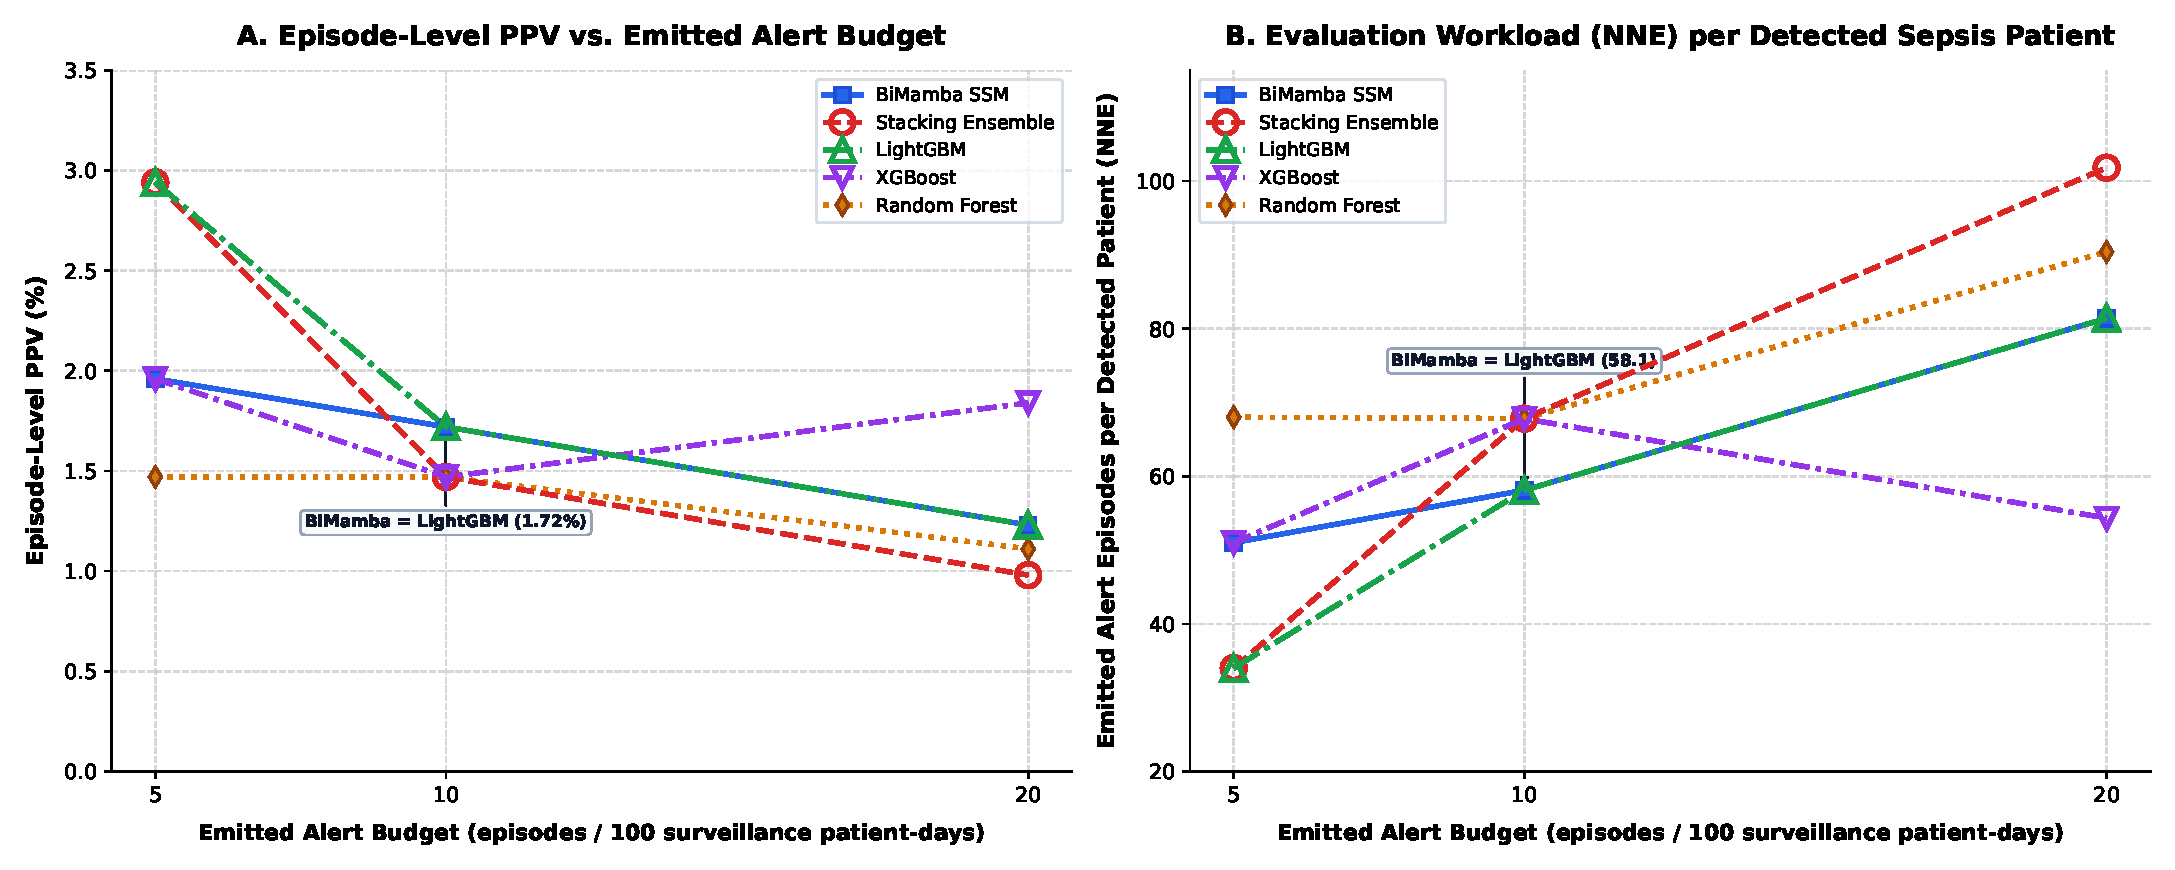
\includegraphics[width=0.90\textwidth]{figures/Figure2_Operational_Alert_Budget_Frontier.pdf}
    \caption{\textbf{Operational Alert-Budget Performance Frontier.} Panel A displays episode-level positive predictive value (PPV \%) across prespecified alert budgets. Panel B displays the Number Needed to Evaluate (NNE) per detected patient under 12h refractory suppression.}
    \label{fig:frontiers}
\end{figure*}

\begin{table*}[t]
\centering
\fontsize{6.3pt}{7.6pt}\selectfont
\setlength{\tabcolsep}{1.8pt}
\caption{\textbf{Operational Burden-Matched Alert Frontiers Under 12h Refractory Suppression.} Evaluated under Procedure B with exposure recomputation and first-emitted-alert timing verification.}
\label{tab:table3}
\begin{tabular*}{\textwidth}{@{\extracolsep{\fill}}llccccccc@{}}
\toprule
\textbf{Budget} & \textbf{Model Architecture} & \textbf{Cutoff ($\tau$)} & \textbf{Alerts ($K$)} & \textbf{Episode PPV \% [95\% CI]} & \textbf{Det ($N$)} & \textbf{Sens. Cov \%} & \textbf{Yield \%} & \textbf{NNE [95\% CI]} \\
\midrule
\textbf{5.0 ep / 100 pt-d} & Stacking Ensemble & 0.0145 & 204 & 2.94 (0.98--5.88)\% & 6 & 3.97 (1.31--7.65)\% & 1.47 (0.49--2.86)\% & 34.0 (17.0--102.0) \\
 & LightGBM & 0.0117 & 204 & 2.94 (0.98--5.39)\% & 6 & 3.97 (1.26--7.10)\% & 1.47 (0.47--2.61)\% & 34.0 (18.5--102.0) \\
 & BiMamba SSM & 0.0187 & 204 & 1.96 (0.49--4.45)\% & 4 & 2.65 (0.65--6.20)\% & 0.98 (0.24--2.31)\% & 51.0 (22.5--204.0) \\
 & XGBoost & 0.0122 & 204 & 1.96 (0.49--3.94)\% & 4 & 2.65 (0.63--5.63)\% & 0.98 (0.23--2.09)\% & 51.0 (25.4--204.0) \\
 & Random Forest & 0.0177 & 204 & 1.47 (0.00--3.45)\% & 3 & 1.99 (0.00--4.49)\% & 0.74 (0.00--1.70)\% & 68.0 (29.0--$\infty$) \\
 & Clinical Transformer & 0.0101 & 204 & 0.98 (0.00--2.46)\% & 2 & 1.32 (0.00--3.50)\% & 0.49 (0.00--1.27)\% & 102.0 (40.6--$\infty$) \\
 & Logistic Regression & 0.0103 & 204 & 0.98 (0.00--2.94)\% & 2 & 1.32 (0.00--3.85)\% & 0.49 (0.00--1.45)\% & 102.0 (34.0--$\infty$) \\
 & Mask-Aware Transformer & 0.0120 & 204 & 0.00 (0.00--0.00)\%$^*$ & 0 & 0.00 (0.00--0.00)\%$^*$ & 0.00 (0.00--0.00)\%$^*$ & Undefined ($\infty$) \\
\midrule
\textbf{10.0 ep / 100 pt-d} & BiMamba SSM & 0.0165 & 407 & 1.72 (0.49--2.95)\% & 7 & 4.64 (1.33--8.16)\% & 1.72 (0.49--2.93)\% & 58.1 (33.9--203.5) \\
 & LightGBM & 0.0110 & 407 & 1.72 (0.49--2.95)\% & 7 & 4.64 (1.38--7.74)\% & 1.72 (0.49--2.89)\% & 58.1 (33.9--203.5) \\
 & Stacking Ensemble & 0.0131 & 407 & 1.47 (0.25--2.46)\% & 6 & 3.97 (0.70--6.98)\% & 1.47 (0.26--2.54)\% & 67.8 (40.7--407.0) \\
 & XGBoost & 0.0114 & 407 & 1.47 (0.49--2.94)\% & 6 & 3.97 (1.32--7.65)\% & 1.47 (0.49--2.85)\% & 67.8 (34.0--203.5) \\
 & Random Forest & 0.0158 & 407 & 1.47 (0.49--2.70)\% & 6 & 3.97 (1.26--7.29)\% & 1.47 (0.47--2.70)\% & 67.8 (37.0--204.0) \\
 & Mask-Aware Transformer & 0.0110 & 407 & 1.23 (0.25--2.46)\% & 5 & 3.31 (0.74--6.67)\% & 1.23 (0.26--2.48)\% & 81.4 (40.7--407.0) \\
 & Clinical Transformer & 0.0094 & 407 & 1.23 (0.25--2.46)\% & 5 & 3.31 (0.68--6.38)\% & 1.23 (0.25--2.37)\% & 81.4 (40.7--407.0) \\
 & Logistic Regression & 0.0095 & 407 & 0.98 (0.25--1.97)\% & 4 & 2.65 (0.59--5.51)\% & 0.98 (0.23--2.07)\% & 101.8 (50.8--408.0) \\
\midrule
\textbf{20.0 ep / 100 pt-d} & XGBoost & 0.0105 & 814 & 1.84 (0.98--2.70)\% & 15 & 9.93 (5.26--14.47)\% & 3.68 (1.87--5.29)\% & 54.3 (37.0--101.9) \\
 & Mask-Aware Transformer & 0.0099 & 814 & 1.72 (0.74--2.58)\% & 14 & 9.27 (4.54--13.77)\% & 3.43 (1.59--5.19)\% & 58.1 (38.8--135.7) \\
 & Logistic Regression & 0.0088 & 814 & 1.35 (0.49--2.09)\% & 11 & 7.28 (2.74--11.11)\% & 2.70 (0.99--4.18)\% & 74.0 (47.8--203.7) \\
 & BiMamba SSM & 0.0142 & 814 & 1.23 (0.49--2.09)\% & 10 & 6.62 (3.07--10.89)\% & 2.45 (1.05--4.10)\% & 81.4 (47.9--203.2) \\
 & LightGBM & 0.0105 & 814 & 1.23 (0.61--2.09)\% & 10 & 6.62 (3.11--11.04)\% & 2.45 (1.15--4.10)\% & 81.4 (47.9--163.0) \\
 & Random Forest & 0.0131 & 814 & 1.11 (0.49--1.85)\% & 9 & 5.96 (2.70--9.68)\% & 2.21 (0.96--3.69)\% & 90.4 (54.2--203.7) \\
 & Stacking Ensemble & 0.0115 & 814 & 0.98 (0.37--1.72)\% & 8 & 5.30 (2.04--9.15)\% & 1.96 (0.74--3.43)\% & 101.8 (58.1--271.3) \\
 & Clinical Transformer & 0.0088 & 814 & 0.86 (0.25--1.48)\% & 7 & 4.64 (1.51--8.18)\% & 1.72 (0.52--3.04)\% & 116.3 (67.8--407.0) \\
\bottomrule
\end{tabular*}
\vspace{0.2em}
\raggedright
\scriptsize
$^*$At zero observed detections, the empirical percentile-bootstrap interval was degenerate at zero. This does not establish zero population detection probability. Fixed-policy binomial reference bounds are provided in the supplement. NNE intervals derived by exact reciprocal transformation. 100\% of detected patients satisfied pre-treatment timing buffers ($\delta=0\text{h}$ and $\delta=2\text{h}$).
\end{table*}

\subsection{Two-Axis Subgroup and Timestamp Uncertainty Matrix}
Table~\ref{tab:table4} presents the cross-tabulation of Sepsis Onset Timing against Treatment Timing. In MIMIC-IV, eMAR administration timestamps verify that 150 of 151 covered patients (99.3\%) and 36.8\% of total incident sepsis episodes had definitive pre-treatment prediction opportunity. In MIMIC-III, prescription start dates lack sub-day precision, creating an interval $[00:00:00, 23:59:59]$ producing 110 indeterminate cases across the cohort, bounding true opportunity between 0.03\% and 3.10\% conditional on assigned consensus onset timestamps.

\begin{table*}[t]
\centering
\fontsize{6.5pt}{7.9pt}\selectfont
\setlength{\tabcolsep}{2.0pt}
\caption{\textbf{Two-Axis Subgroup and Timestamp Uncertainty Matrix.} Opportunity bounds conditional on fixed consensus Sepsis-3 timestamps and surveillance coverage.}
\label{tab:table4}
\begin{tabular*}{\textwidth}{@{\extracolsep{\fill}}llcccccc@{}}
\toprule
\textbf{Cohort \& Timestamp Source} & \textbf{Sepsis Onset Category} & \textbf{Total ($N$)} & \textbf{Covered ($V=1$)} & \textbf{Eligible ($O=1$)} & \textbf{Indeterminate} & \textbf{Subgroup Bounds} & \textbf{Contribution to Cohort} \\
\midrule
\textbf{MIMIC-IV Prospective-Replay} & Early Incident ($\le 24\text{h}$) & 47 & 47 (100.0\%) & 47 & 0 & [100.0\%, 100.0\%] & 47 / 408 (11.5\%) \\
\textit{(Hourly Confirmed eMAR)} & Intermediate (24--48h) & 156 & 104 (66.7\%) & 103 & 0 & [66.0\%, 66.0\%] & 103 / 408 (25.2\%) \\
 & Late Incident ($>48\text{h}$) & 205 & 0 (0.0\%) & 0 & 0 & [0.0\%, 0.0\%] & 0 / 408 (0.0\%) \\
 & \textbf{All Incident Sepsis-3} & \textbf{408} & \textbf{151 (37.0\%)} & \textbf{150} & \textbf{0} & \textbf{[36.8\%, 36.8\%]} & \textbf{150 / 408 (36.8\%)} \\
\midrule
\textbf{MIMIC-III Broad Incident Sepsis} & Early Incident ($\le 24\text{h}$) & 2,641 & 102 (3.9\%) & 0 & 74 & [0.0\%, 2.8\%] & [0, 74] / 3,581 (0.00--2.07\%) \\
\textit{(Date-Level Prescription Proxy)} & Intermediate (24--48h) & 361 & 235 (65.1\%) & 1 & 36 & [0.3\%, 10.2\%] & [1, 37] / 3,581 (0.03--1.03\%) \\
 & Late Incident ($>48\text{h}$) & 579 & 0 (0.0\%) & 0 & 0 & [0.0\%, 0.0\%] & [0, 0] / 3,581 (0.00\%) \\
 & \textbf{All Incident Sepsis-3} & \textbf{3,581} & \textbf{337 (9.4\%)} & \textbf{1} & \textbf{110} & \textbf{[0.03\%, 3.10\%]} & \textbf{[1, 111] / 3,581 (0.03--3.10\%)} \\
\bottomrule
\end{tabular*}
\end{table*}

\subsection{Cumulative Population Coverage Decomposition}
Figure~\ref{fig:decomp} illustrates the cumulative population coverage decomposition:
\[
\frac{151}{408} \times \frac{150}{151} \times \frac{7}{150} = \frac{7}{408} = 1.72\%
\]
\begin{enumerate}
    \item \textbf{Surveillance Truncation ($151/408 = 37.0\%$):} 63.0\% of sepsis patients develop onset after hour 36, outside the prespecified second-day surveillance protocol.
    \item \textbf{Pretreatment Actionability ($150/151 = 99.3\%$):} Among covered stays, treatment almost never occurs prior to surveillance lookback windows.
    \item \textbf{Workload Detection Yield ($7/150 = 4.67\%$):} Under an alert budget of 10 episodes/100 patient-days, BiMamba SSM detects 7 patients (1.72\% whole-population yield; NNE = 58.1).
\end{enumerate}

\begin{figure}[t]
    \centering
    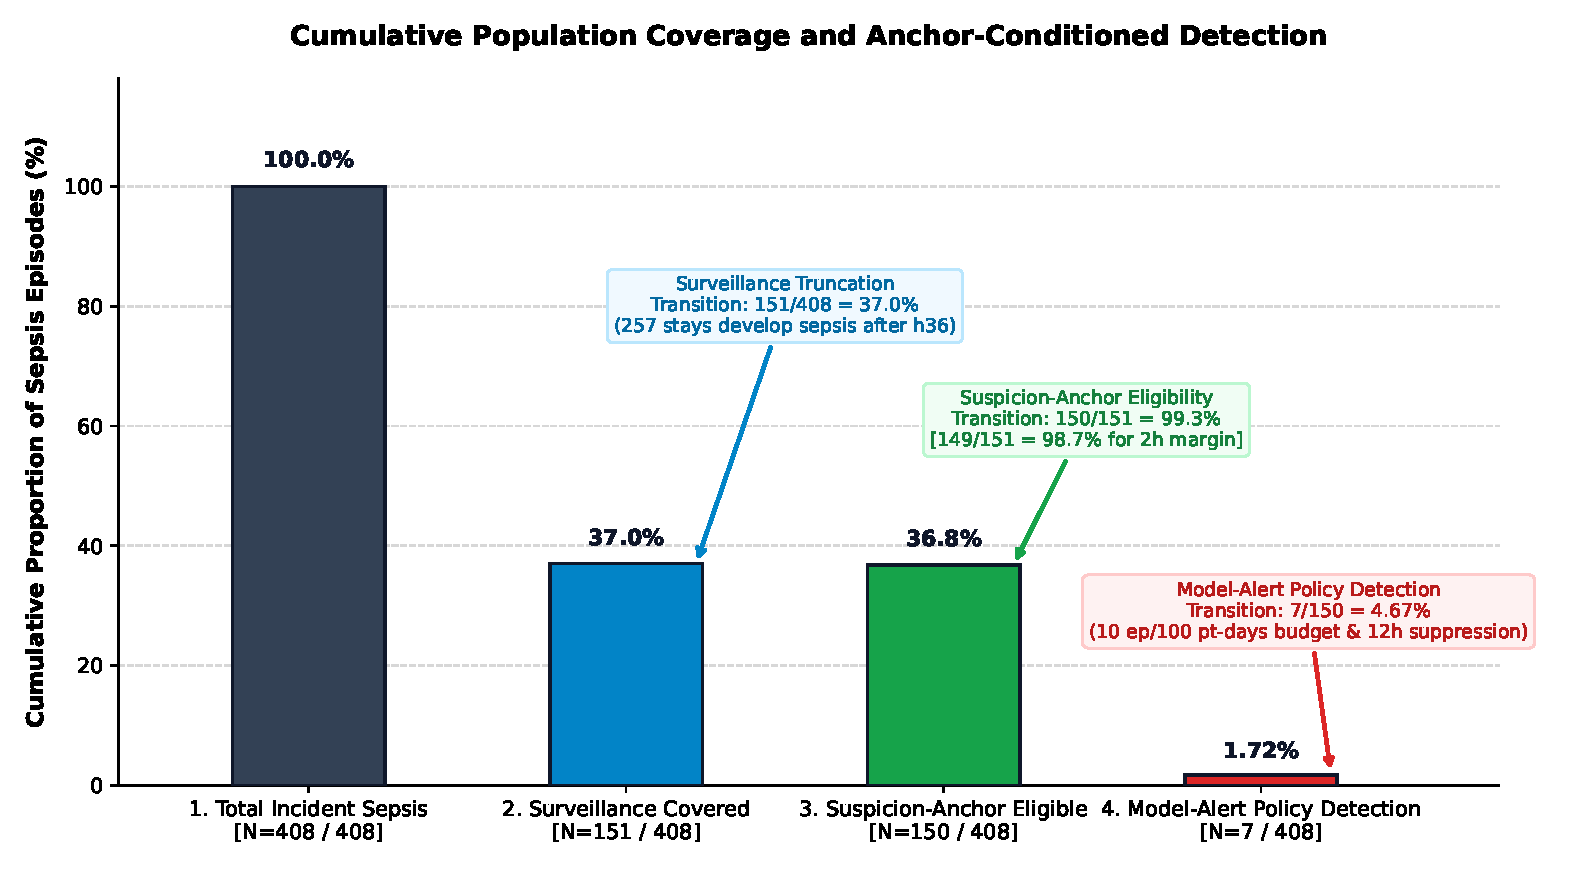
\includegraphics[width=\columnwidth]{figures/Figure3_Three_Stage_Decomposition.pdf}
    \caption{\textbf{Cumulative Population Coverage and Actionability Decomposition.} Stepwise attrition from 408 incident sepsis episodes through protocol coverage, pre-treatment opportunity, and alert-budget detection.}
    \label{fig:decomp}
\end{figure}

\section{Discussion}
The central finding of this investigation resolves the paradox between retrospective discriminative benchmarks and prospective bedside failures:
\begin{enumerate}
    \item \textbf{Pre-treatment Discrimination Is Preserved:} In directional consistency with Dutta et al. (2026), model discrimination (AUROC) does not collapse when evaluating true pre-treatment sepsis detection on risk sets excluding post-treatment windows. Models are capable of identifying physiological derangements ahead of antimicrobial intervention.
    \item \textbf{The Bottleneck Is Operational and Workload-Driven:} When models operate under realistic clinical alert budgets ($\le 10$ alert episodes per 100 patient-days), whole-population sensitivity is bounded below 2\%, with PPV between 1.0\% and 1.7\%, requiring 58.1 to 67.8 bedside reviews per detected patient.
    \item \textbf{Surveillance Protocol Truncation Explains Missing Cases:} Sepsis in critical care does not adhere to narrow 12-hour evaluation windows; median onset occurs 49 hours into admission. In second-day surveillance protocols, over 60\% of cases develop onset after the monitoring window terminates.
\end{enumerate}

A critical conceptual error in prior literature is \textbf{endpoint substitution}. When benchmarks predict ``antibiotic initiation within 6 hours across all patients'', they evaluate care-process prediction (predicting clinician ordering behavior, including prophylactic prescribing in non-septic patients). This task is fundamentally distinct from pre-treatment sepsis detection. Machine learning benchmarks must maintain Sepsis-3 as the biological target while conditioning evaluation timestamps on decision availability.

\subsection{Limitations}
This study evaluated a prespecified second-day ICU surveillance protocol (hours 19--30); full-stay prospective surveillance across multiple hospital systems remains essential to establish multi-center transportability. Furthermore, MIMIC-III prescription start dates exhibit substantial interval uncertainty, necessitating primary reliance on MIMIC-IV confirmed eMAR records.

\subsection{Conclusion}
In this restricted, long-stay ICU cohort, observed detection yield depended on surveillance coverage, discrimination, and the policy used to constrain emitted alerts. Most horizon-positive observations remained pretreatment eligible, and model rankings varied across workload levels. Deployable sepsis early-warning systems require benchmarking under locked alert budgets, deduplicating refractory alert workload, and enforcing multi-clock reporting.

\section*{Code and Data Availability}
All preprocessing pipelines, model architectures, evaluation harnesses, and release manifests are publicly available under MIT License at \url{https://github.com/alireza/Sepsis-Onset-Timing-Paradox} (Git commit \texttt{b0932ca}, manifest \texttt{1.0.0-freeze}). De-identified patient data are available from PhysioNet under the MIMIC-IV Data Use Agreement.

\begin{thebibliography}{10}
\bibitem{singer2016sepsis} Singer M, Deutschman CS, Seymour CW, et al. The third international consensus definitions for sepsis and septic shock (Sepsis-3). \textit{JAMA}. 2016;315(8):801--810.
\bibitem{seymour2016assessment} Seymour CW, Liu VX, Iwashyna TJ, et al. Assessment of clinical criteria for sepsis: for the Third International Consensus Definitions for Sepsis and Septic Shock (Sepsis-3). \textit{JAMA}. 2016;315(8):762--774.
\bibitem{weissman2024sepsis} Weissman GE, et al. Sepsis prediction models diverge from clinician treatment times. \textit{AMIA Annu Symp Proc}. 2024;2024:1215--1224.
\bibitem{wong2021external} Wong A, Otles E, Donnelly JP, et al. External validation of a widely implemented proprietary sepsis prediction model in hospitalized patients. \textit{JAMA Intern Med}. 2021;181(8):1065--1070.
\bibitem{dutta2026performance} Dutta S, et al. Performance of sepsis prediction across operational definitions. \textit{JAMA Netw Open}. 2026;9(3):e265599.
\bibitem{kumar2006duration} Kumar A, Roberts D, Wood KE, et al. Duration of hypotension before initiation of effective antimicrobial therapy is the critical determinant of survival in human septic shock. \textit{Crit Care Med}. 2006;34(6):1589--1596.
\bibitem{moor2023foundation} Moor M, Banerjee O, Abad ZSH, et al. Foundation models for generalist medical artificial intelligence. \textit{Nature}. 2023;616(7956):259--265.
\bibitem{collins2024tripod} Collins GS, Moons KG, Dhiman P, et al. TRIPOD+AI statement: updated guidance for reporting clinical prediction models that use machine learning. \textit{BMJ}. 2024;385:e078378.
\bibitem{johnson2016mimic} Johnson AE, Pollard TJ, Shen L, et al. MIMIC-III, a freely accessible critical care database. \textit{Sci Data}. 2016;3:160035.
\end{thebibliography}

\end{document}
